% !TEX root = ../main.tex
% File: chapters_part1/chap6_5.tex
% Nội dung cho Chương 6, Phần 5

\section{Mô hình Thế giới (World Models) và Mô phỏng}
\label{sec:world_models}

Khi chúng ta đi đến cuối chương về các hệ thống nâng cao, một câu hỏi sâu sắc và cơ bản được đặt ra: Khi một LLM dự đoán từ tiếp theo một cách chính xác trên một lượng dữ liệu khổng lồ, nó thực sự đang học được điều gì? Liệu nó có chỉ đơn thuần học các quy luật thống kê bề mặt của ngôn ngữ, hay nó đang âm thầm xây dựng một thứ gì đó sâu sắc hơn -- một \textbf{mô hình nội tại (internal model)} về thế giới mà ngôn ngữ đó mô tả?

Đây chính là ý tưởng cốt lõi đằng sau khái niệm \textbf{Mô hình Thế giới (World Models)}.

\subsection{Khái niệm về khả năng LLM xây dựng mô hình nội tại}
\label{ssec:internal_world_model_concept}

\begin{definition}{Mô hình Thế giới (trong bối cảnh LLM)}{def:world_model}
    Một Mô hình Thế giới là một biểu diễn nén, có thể thực thi (executable), và trừu tượng về các thực thể, mối quan hệ, và các quy luật vật lý/xã hội của thế giới, được hình thành bên trong các trọng số của một mô hình ngôn ngữ lớn thông qua quá trình huấn luyện trên dữ liệu văn bản.
\end{definition}

\begin{tcolorbox}[
    title=Triết lý của Mô hình Thế giới,
    colback=blue!5!white, colframe=blue!75!black, fonttitle=\bfseries
]
Giả thuyết cho rằng: để có thể dự đoán văn bản một cách hiệu quả và nhất quán trên nhiều lĩnh vực, cách tối ưu nhất cho mô hình không phải là ghi nhớ tất cả các chuỗi ký tự, mà là xây dựng một mô hình nén của các quy luật sinh ra văn bản đó. Vì văn bản là sự phản ánh của thế giới, nên một mô hình tốt của văn bản cũng phải là một mô hình tốt của thế giới.
\end{tcolorbox}

\subsubsection{Các bằng chứng gián tiếp}
Mặc dù chúng ta không thể "nhìn" trực tiếp vào các trọng số và thấy một "mô hình thế giới" rõ ràng, có nhiều bằng chứng gián tiếp cho thấy các LLM lớn đang học được những biểu diễn như vậy:
\paragraph{Biểu diễn không gian và thời gian}
\begin{itemize}
    \item Các nhà nghiên cứu đã phát hiện ra các nơ-ron hoặc các hướng (directions) trong không gian kích hoạt của LLM dường như tương ứng với các khái niệm trong thế giới thực. Ví dụ, có những nơ-ron chỉ "kích hoạt" mạnh khi mô hình xử lý các văn bản liên quan đến một địa điểm địa lý cụ thể như "Tháp Eiffel" hoặc một mốc thời gian cụ thể.
    \item Yann LeCun đã đưa ra ví dụ: để dự đoán từ cuối cùng trong câu "John cầm quả bóng, đi vào phòng khách, đặt quả bóng xuống, rồi đi vào bếp. Quả bóng đang ở...", mô hình phải có một biểu diễn nội tại về không gian, về các đối tượng và vị trí của chúng.
\end{itemize}

\paragraph{Mô phỏng các thực thể}
\begin{itemize}
    \item Khi một LLM tương tác trong một vai trò (ví dụ: "hãy đóng vai Napoleon"), nó có thể duy trì sự nhất quán về kiến thức, tính cách, và các mối quan hệ của nhân vật đó trong một cuộc hội thoại dài. Điều này cho thấy nó không chỉ lấy ra các thông tin rời rạc, mà dường như đang "mô phỏng" một mô hình về thực thể "Napoleon".
\end{itemize}

\paragraph{Mô hình Othello-GPT}
Một nghiên cứu nổi tiếng đã huấn luyện một Transformer nhỏ chỉ để chơi cờ Othello (cờ lật). Mô hình chỉ nhận vào chuỗi các nước đi hợp lệ và dự đoán nước đi hợp lệ tiếp theo.
\begin{itemize}
    \item \textbf{Kết quả đáng kinh ngạc:} Sau khi huấn luyện, các nhà nghiên cứu đã tìm thấy một biểu diễn rõ ràng của \textbf{trạng thái bàn cờ Othello} bên trong các kích hoạt của mô hình. Tức là, mô hình đã tự học cách xây dựng một "mô hình thế giới" (bàn cờ) để có thể chơi tốt, mặc dù nó chưa bao giờ được "nhìn thấy" bàn cờ một cách trực tiếp.
\end{itemize}

\begin{center}
    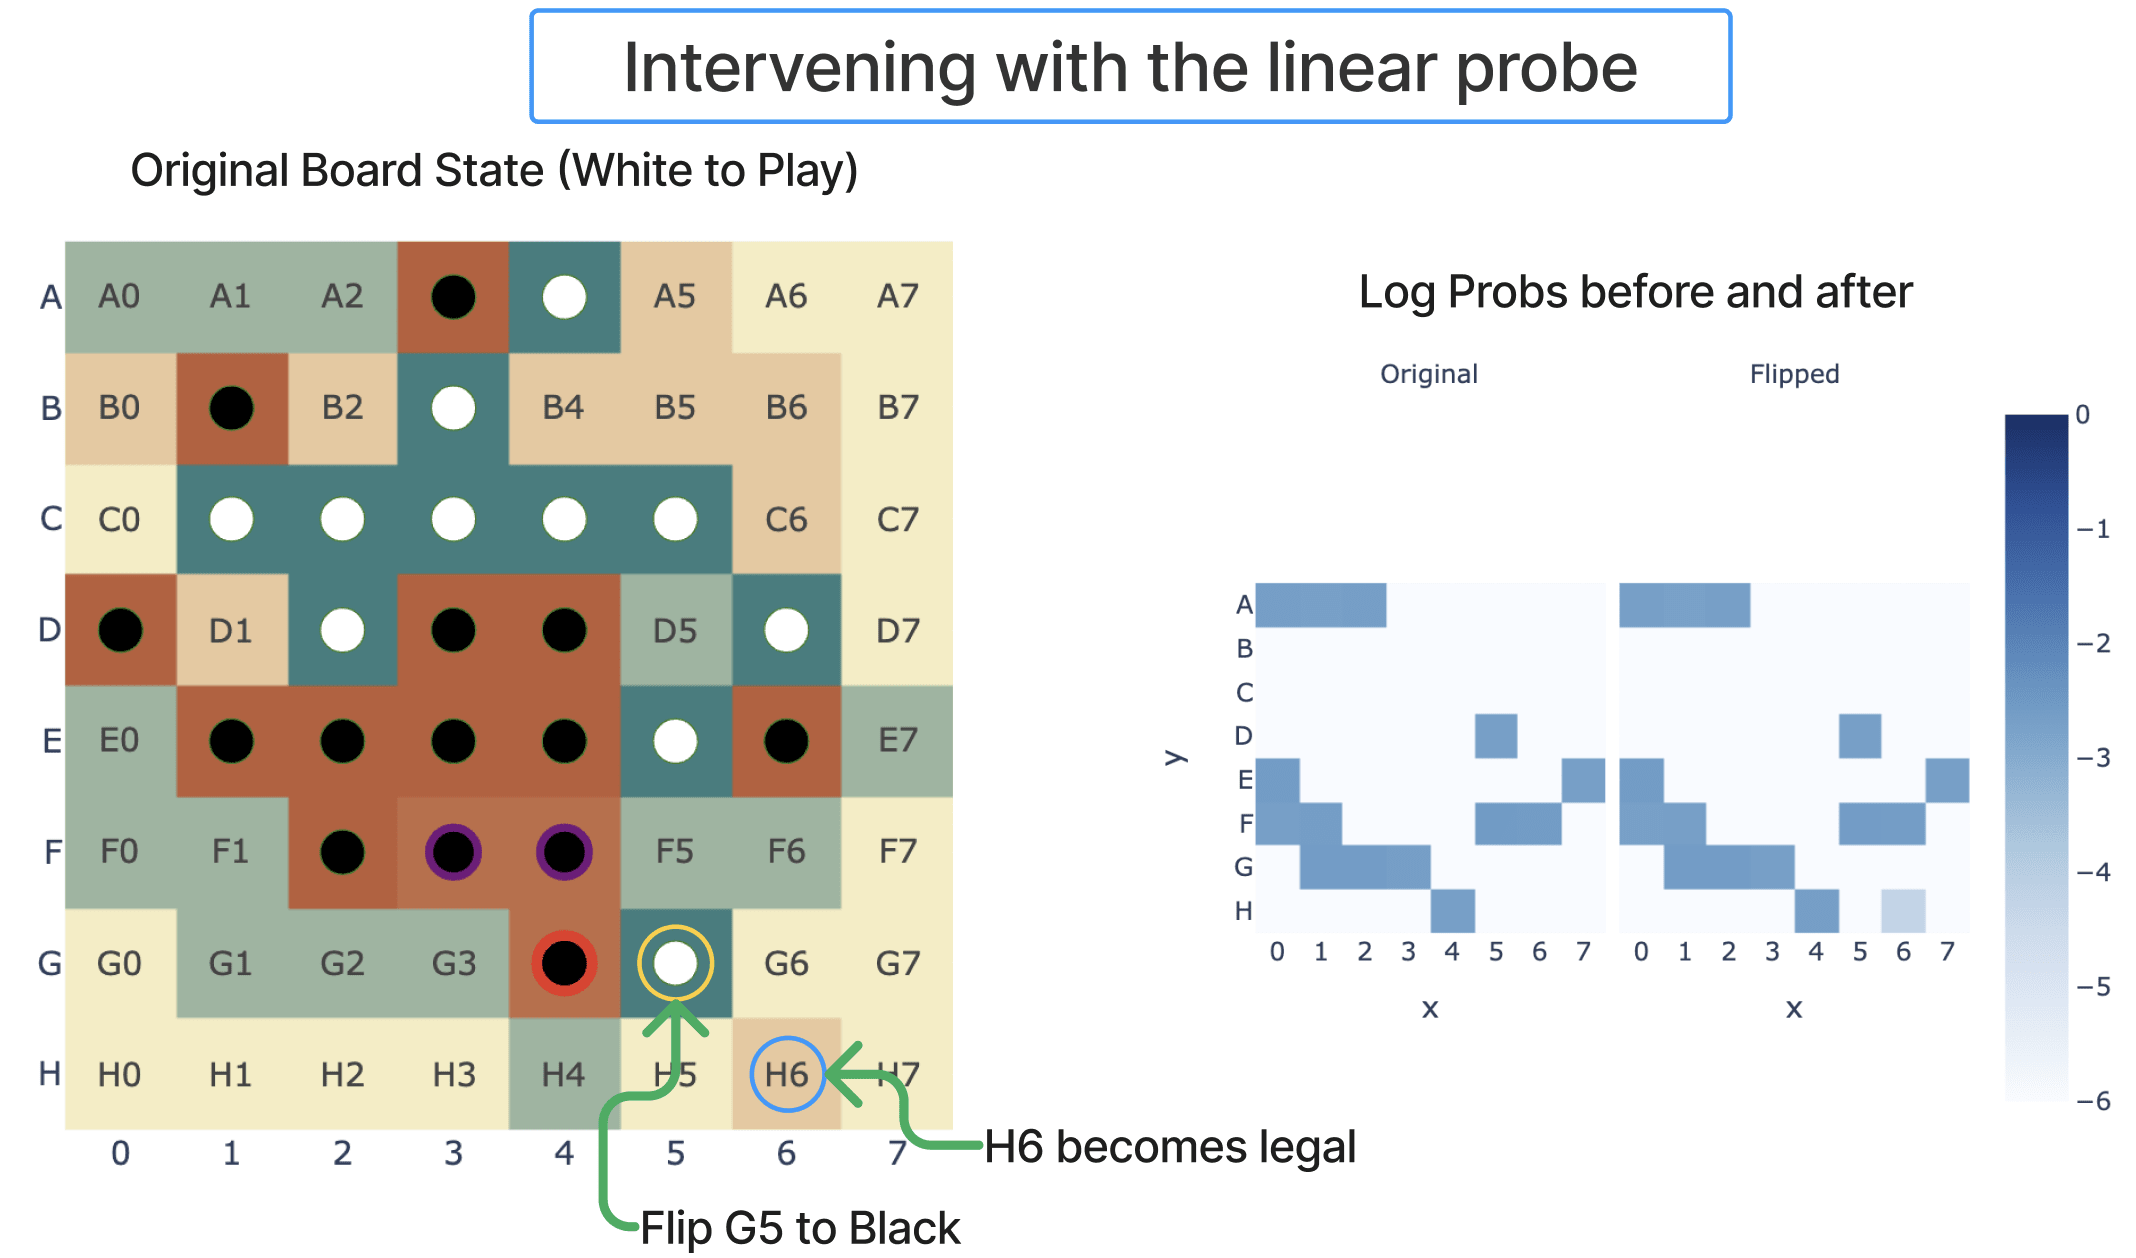
\includegraphics[width=0.7\textwidth]{othello_gpt.png}
    \captionof{figure}{Nghiên cứu Othello-GPT cho thấy một mô hình Transformer, chỉ được huấn luyện trên chuỗi nước đi, đã tự học cách biểu diễn trạng thái của bàn cờ bên trong nó.}
    \label{fig:othello_gpt}
\end{center}

\subsection{Hướng nghiên cứu và Tiềm năng}
\label{ssec:world_models_future}
Việc các LLM có thể xây dựng mô hình thế giới nội tại mở ra những hướng đi cực kỳ hứa hẹn cho tương lai của AI.

\subsubsection{Cải thiện khả năng Suy luận và Lập kế hoạch}
\begin{itemize}
    \item Nếu một Tác tử AI có một mô hình thế giới nội tại tốt, nó có thể thực hiện "mô phỏng trong tâm trí" (mental simulation).
    \item Trước khi thực hiện một hành động trong thế giới thực, nó có thể "chạy thử" hành động đó trên mô hình thế giới của mình để dự đoán kết quả.
    \item Điều này cho phép nó lập kế hoạch một cách hiệu quả hơn nhiều, lường trước các hậu quả, và tránh các sai lầm tốn kém, tương tự như cách con người suy nghĩ "nếu... thì...".
\end{itemize}

\subsubsection{Mô hình Thế giới Đa phương thức}
\begin{itemize}
    \item Hướng nghiên cứu hiện tại đang tập trung vào việc xây dựng các mô hình thế giới không chỉ từ văn bản, mà còn từ \textbf{video}.
    \item Bằng cách xem hàng triệu giờ video, một mô hình có thể học được các quy luật vật lý trực quan (intuitive physics) -- ví dụ, một vật thể không thể đi xuyên qua vật thể khác, trọng lực làm cho mọi thứ rơi xuống.
    \item Các mô hình như \textbf{Sora} của OpenAI, có khả năng sinh ra các video cực kỳ thực tế và nhất quán về mặt vật lý, được cho là một bước tiến lớn trong việc xây dựng các mô hình thế giới có khả năng mô phỏng.
\end{itemize}

\subsubsection{Hướng tới Trí tuệ Nhân tạo Tổng quát (AGI)}
\begin{itemize}
    \item Nhiều nhà nghiên cứu hàng đầu tin rằng khả năng xây dựng và sử dụng các mô hình thế giới là một trong những thành phần cốt lõi của trí thông minh thực sự.
    \item Một hệ thống AGI trong tương lai có thể sẽ bao gồm một LLM lớn đóng vai trò là "giao diện" ngôn ngữ, kết hợp với một mô hình thế giới mạnh mẽ cho phép nó hiểu sâu, suy luận, và lập kế hoạch trong một môi trường phức tạp.
\end{itemize}

Mặc dù vẫn còn là một lĩnh vực đầy tranh cãi và câu hỏi mở, giả thuyết về Mô hình Thế giới cung cấp một lăng kính mạnh mẽ để hiểu về những khả năng đáng kinh ngạc của LLM. Nó gợi ý rằng chúng ta có thể đang vô tình xây dựng được những thứ phức tạp hơn nhiều so với những gì chúng ta nghĩ ban đầu, mở ra một tương lai đầy tiềm năng cho các hệ thống AI có khả năng lý luận và tương tác với thế giới một cách sâu sắc.